\documentclass[12pt,letterpaper]{exam}
\usepackage[lmargin=1in,rmargin=1in,tmargin=1in,bmargin=1in]{geometry}
\usepackage{../style/exams}

% -------------------
% Course & Exam Information
% -------------------
\newcommand{\course}{MAT 100: Exam 2}
\newcommand{\term}{Fall -- 2021}
\newcommand{\examdate}{12/13/2021}
\newcommand{\timelimit}{85 Minutes}

\setbool{hideans}{true} % Student: True; Instructor: False

% -------------------
% Content
% -------------------
\begin{document}

\examtitle
\instructions{Write your name on the appropriate line on the exam cover sheet. This exam contains \numpages\ pages (including this cover page) and \numquestions\ questions. Check that you have every page of the exam. Answer the questions in the spaces provided on the question sheets. Be sure to answer every part of each question and show all your work.} 
\scores
\bottomline
\newpage

% ---------
% Questions
% ---------
\begin{questions}

% Question 1
\newpage
\question[5] Sketch the quadratic function $f(x)= 4 - (x + 3)^2$ in the graph below. Your sketch should include the vertex and axis of symmetry for $f(x)$. 
	\[
	\fbox{
	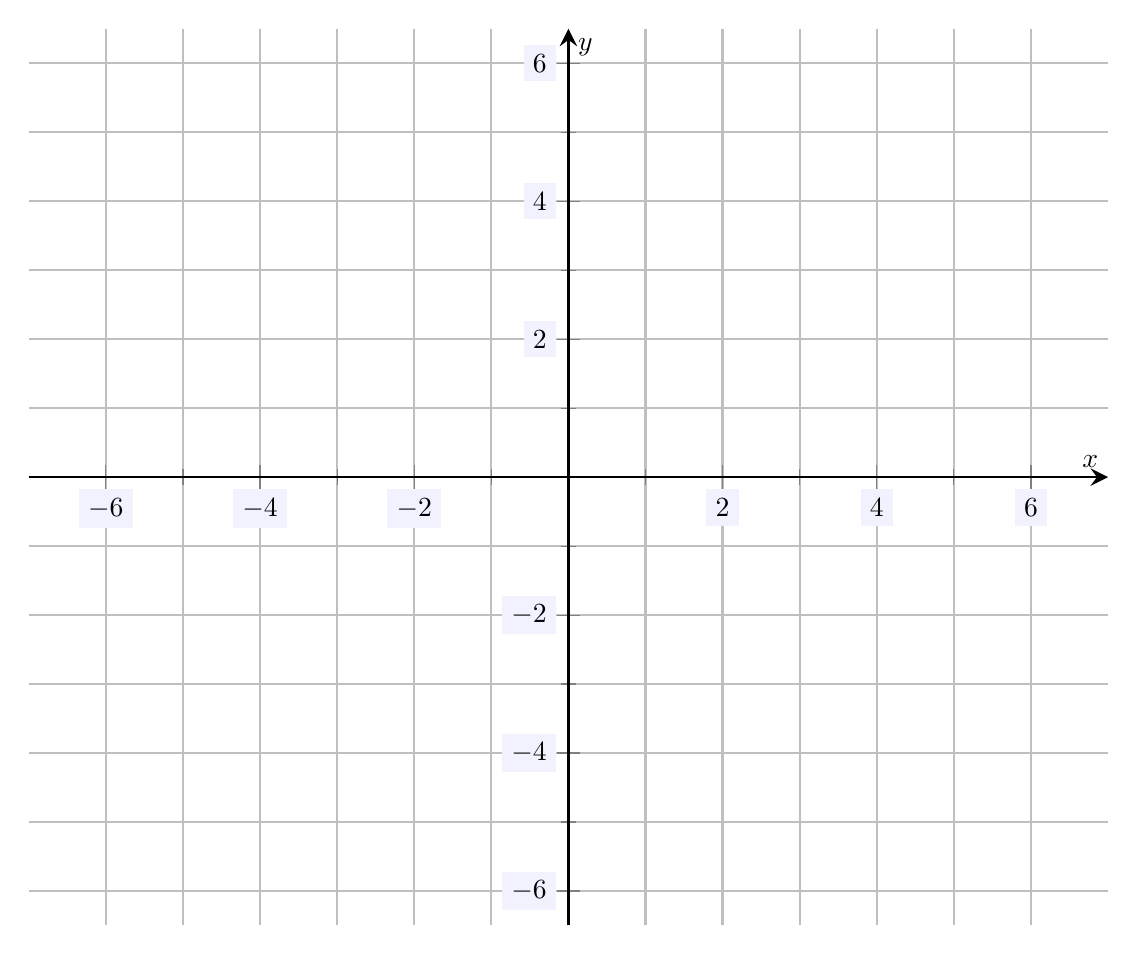
\begin{tikzpicture}[scale=2,every node/.style={scale=0.5}]
	\begin{axis}[
	grid=both,
	axis lines=middle,
	ticklabel style={fill=blue!5!white},
	xmin= -7, xmax=7,
	ymin= -6.5, ymax=6.5,
	xtick={-6,-4,-2,0,2,4,6},
	ytick={-6,-4,-2,0,2,4,6},
	minor tick = {-5,-3,...,5},
	xlabel=\(x\),ylabel=\(y\),
	]
	\end{axis}
	\end{tikzpicture}
	}
	\]





% Question 2
\newpage
\question[10] Let $f(x)$ be the quadratic function $f(x)= 5x^2 + 10x - 7$.
\begin{enumerate}[(a)]
\item Find the vertex and axis of symmetry for $f(x)$.
\item Does this parabola open upwards or downwards? Explain.
\item Is the function convex or concave? 
\item Does the function have a maximum or minimum value? Explain. 
\item Find the maximum or minimum value from (d). 
\end{enumerate}





% Question 3
\newpage
\question[5] Find the vertex form of $y= x^2 - 8x + 21$. 





% Question 4
\newpage
\question[5] Factor the polynomial $x^2 - 16x + 55$.





% Question 5
\newpage
\question[5] Factor the polynomial $x^2 - 2x - 48$. 





% Question 6
\newpage
\question[5] Factor the polynomial $2x^2 + 3x - 30$. 





% Question 7
\newpage
\question[5] Consider the function $f(x)= x^2 + 2x - 8$. Find the $x$ and $y$ intercepts for this function. 





% Question 8
\newpage
\question[5] Find the solutions to $6x - x^2= 9$. 





% Question 9
\newpage
\question[5] Find the solutions to $x^2= x + 20$. 





% Question 10
\newpage
\question[5] Using the quadratic equation, find the solutions to $x^2 - 2x - 7= 0$. 





% Question 11
\newpage
\question[10] Consider the rational function $f(x)= \dfrac{x^2 - 9}{x^2 + 2x - 15}$. 
\begin{enumerate}[(a)]
\item Find the domain for $f(x)$. 
\item Find the vertical asymptotes for $f(x)$. 
\item Find the zeros for $f(x)$. 
\end{enumerate}





% Question 12
\newpage
\question[5] Compute the following, being sure to simplify as much as possible: 
	\[
	\dfrac{3}{x^2 - 4} - \dfrac{x - 1}{x^2 - x - 2}
	\]





% Question 13
\newpage
\question[5] Compute the following, being sure to simplify as much as possible:
	\[
	\dfrac{x^2 - 2x - 3}{x^2 + 6x - 7} \cdot \dfrac{x^2 + 9x + 14}{x^2 + 5x + 4} 
	\]





% Question 14
\newpage
\question[5] Compute the following, begin sure to simplify as much as possible:
	\[
	\dfrac{\phantom{--}\dfrac{x^2 + 5x}{x^2 - 1}\phantom{--}}{\dfrac{x^2 + 3x - 10}{x^2 + 8x - 9}}
	\]





% Question 15
\newpage
\question[5] Solve the following system of equations:
	\[
	\begin{aligned}
	x + y&= 4 \\
	x - y&= 10
	\end{aligned}
	\]





% Question 16
\newpage
\question[5] Solve the following system of equations: 
	\[
	\begin{aligned}
	2x - 3y&= 4 \\
	6x - 2y&= 5
	\end{aligned}
	\]





% Question 17
\newpage
\question[5] Determine whether the point $(1, -5)$ is a solution to the following system of equations:
	\[
	\begin{aligned}
	5x - y&= 10 \\
	x + y&= 0 
	\end{aligned}
	\]





% Question 18
\newpage
\question[5] Explain why the following system of equations does not have a solution. Be sure to justify your answer. 
	\[
	\begin{aligned}
	-6x + y&= 3 \\
	12x - 2y&= -4
	\end{aligned}
	\]


\end{questions}
\end{document}